\documentclass{standalone}
\usepackage{standalone}

\begin{document}
\subsection{Plate and regions extraction}
This step extracts the license plate and its bounding regions primarily. This does not detect actual license plate. But gives a close approximation to the location of the license plate. First we calculated all contours of the image calculated by mixture model. Next for each contours, we validated the bounding rectangle it is in. If the size of the bounding rectangle is valid, we extract the image of the area and region data. The extracted plates from the previous stage is shown in Figure \ref{fig:ExtractedPlates}.

\begin{figure}
\begin{subfigure}{.5\textwidth}
  \centering
  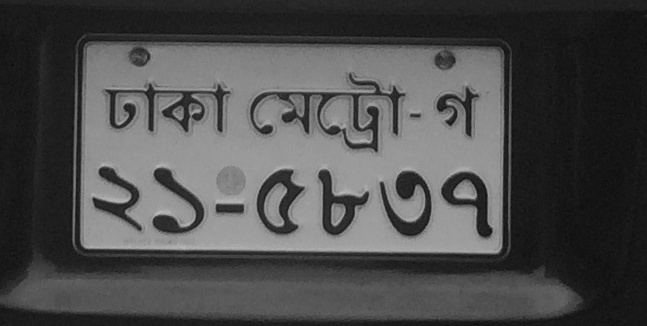
\includegraphics[width=.8\linewidth]{./img/sample/stage6-1.jpg}
  \caption{First estimation}
  \label{fig:FirstExtracted}
\end{subfigure}
\begin{subfigure}{.5\textwidth}
  \centering
  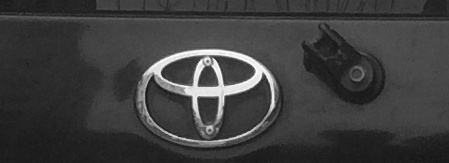
\includegraphics[width=.8\linewidth]{./img/sample/stage6-2.jpg}
  \caption{Second estimation}
  \label{fig:SecondExtracted}
\end{subfigure}
\begin{subfigure}{.5\textwidth}
  \centering
  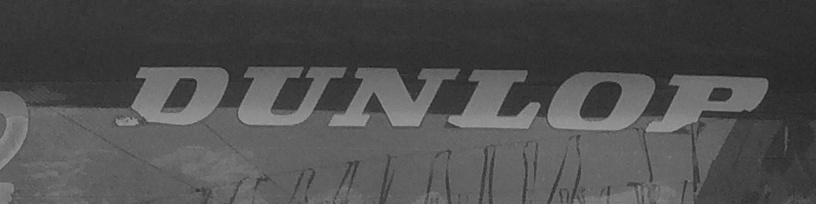
\includegraphics[width=.8\linewidth]{./img/sample/stage6-3.jpg}
  \caption{Third estimation}
  \label{fig:ThirdExtracted}
\end{subfigure}
\begin{subfigure}{.5\textwidth}
  \centering
  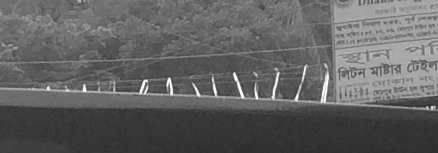
\includegraphics[width=.8\linewidth]{./img/sample/stage6-4.jpg}
  \caption{Fourth estimation}
  \label{fig:FourthExtracted}
\end{subfigure}
\caption{Estimated license plates.}
\label{fig:ExtractedPlates}
\end{figure}

\end{document}